%---------------------------------------------------------------------------
\chapter{\Introspection}
%----------------------------------------------------------------------------
\section{A teszt bemutatása és célja}
%----------------------------------------------------------------------------

A 84 kérdésből álló PAMS önértékelő kérdőív kitöltésével saját vezetői 
és személyes kompetenciáimat szerettem volna feltérképezni.
A teszt három fő területre fókuszál: egyéni, személyközi és csoportos készségekre.
Célom az volt, hogy reális képet kapjak arról, milyen erősségekkel rendelkezem vezetőként, 
és mely területeken érdemes még fejlődnöm. A kitöltött tesztet a dolgozat mellékletében csatoltam.

A kérdőív 1-től 6-ig terjedő skálán értékeli az egyes kompetenciákat, ahol a 6-os a legmagasabb szintet jelöli.
A válaszaim túlnyomó része 6-os értéket kapott, ami azt jelzi, hogy tudatosan törekszem a fejlődésre, 
és már most is erős önismerettel, következetességgel és felelősségvállalással dolgozom.

%----------------------------------------------------------------------------
\section{Általános értékelés}
%----------------------------------------------------------------------------

Összességében az eredmények alapján magas szintű vezetői és személyes kompetenciákkal rendelkezem.
Különösen erősnek érzem magam a kommunikáció, a problémamegoldás, a csapatvezetés és az innovatív gondolkodás területein.
A legtöbb válasz esetében 6-os értéket adtam, ami azt tükrözi, hogy stabilan, tudatosan és értékalapúan működöm.
A céljaimat rendszerint végigviszem, képes vagyok másokat motiválni, és jól reagálok stresszes vagy változó helyzetekben is.

%----------------------------------------------------------------------------
\section{Részletes kompetenciaelemzés}
%----------------------------------------------------------------------------

\subsection{Önismeret és személyes hatékonyság}

Fontosnak tartom az önreflexiót és az önismeretet, hiszen ezek nélkül nem lehet hatékonyan vezetni.
Tisztában vagyok az erősségeimmel és a korlátaimmal is, és nem félek a visszajelzésektől.
Igyekszem folyamatosan fejleszteni magam, tanulni a tapasztalataimból, 
és javítani azokon a területeken, ahol érzem, hogy van még hova fejlődni.

\subsection{Stresszkezelés és időgazdálkodás}

Úgy érzem, jól kezelem a stresszt, és tudatosan figyelek arra, hogy ne csak hatékonyan dolgozzak, hanem regenerálódjak is.
A feladataimat igyekszem mindig priorizálni, és nem hagyom, hogy a felesleges terhelés elvigye az energiámat.
Viszont elismerem, hogy a pihenésre és kikapcsolódásra néha több 
figyelmet kellene fordítanom, mert hajlamos vagyok túlvállalni magam, ha fontos projektről van szó.

\subsection{Problémamegoldás és döntéshozatal}

Erősségemnek tartom a rendszerszintű és logikus gondolkodást.
Döntéseimet nem hirtelen hozom meg, hanem mindig több lehetőséget mérlegelek, és igyekszem a legjobb megoldást választani.
Ugyanakkor nem félek kockázatot vállalni, ha azt érzem, hogy az a fejlődés vagy a csapat érdekeit szolgálja.
A kreatív gondolkodás nálam természetes része a problémamegoldásnak, de tudatosan figyelek arra is, 
hogy a megoldások ne csak innovatívak, hanem kivitelezhetők is legyenek.

\subsection{Kreativitás és innováció}

A munkám során sokszor kerülök olyan helyzetbe, ahol gyorsan, kreatívan kell reagálni.
Szeretek új megoldásokat kipróbálni, akár technikai, akár szervezési szinten.
Fontosnak tartom, hogy a csapatom is merjen kísérletezni és fejlődni, mert hiszek abban, 
hogy az innováció csak így születhet meg, ettől lesz egyedi és versenyképes egy csapat vagy szervezet.

\subsection{Kommunikáció és visszajelzés}

A kommunikáció mindig is központi szerepet játszott a munkámban, és a magánéletemben is.
Törekszem arra, hogy világosan, érthetően és empatikusan kommunikáljak, akár egy csapattaggal, akár ügyféllel beszélek.
A visszajelzéseket nem csak adom, hanem kérem is, mert ezekből tudok tanulni.
Fontos számomra, hogy a problémákat mindig nyíltan, őszintén, 
de tisztelettel kezeljem - ez szerintem az egyik legfontosabb vezetői kompetencia, amit sikerült tudatosan kialakítanom.

\subsection{Motiváció és teljesítménymenedzsment}

A csapat motiválása nálam elsősorban emberi kapcsolatokon és példamutatáson alapul.
Sokszor személyesen is próbálok inspirálni másokat, nemcsak utasításokkal, hanem bizalommal és támogatással.
Bevallom, a formális jutalmazási rendszert kevésbé alkalmazom, mert inkább 
a szakmai elismerésben és a fejlődés lehetőségében hiszek.
Ugyanakkor érzem, hogy ezen a területen érdemes lenne tudatosabban használni 
a jutalmazás és elismerés eszközeit, mert ez még hatékonyabbá teheti a csapatműködést.

\subsection{Csapatvezetés és együttműködés}

Szeretek csapatban dolgozni, és hiszek abban, hogy a legjobb eredmények mindig közösen születnek.
Tudatosan figyelek arra, hogy mindenki értse a célokat, és lássa, miért fontos a saját szerepe a közös sikerben.
Nyitott vagyok a véleményekre, és igyekszem olyan légkört teremteni, ahol mindenki bátran megoszthatja a gondolatait.
A csapatvezetés terén stabilnak érzem magam, mert nemcsak irányítok, hanem fejlesztek és támogatok is.

\subsection{Változáskezelés és inspiráció}

Hiszek abban, hogy a vezetés nem a hatalomról, hanem a példamutatásról és a hatásról szól.
A változásokat nem kényszerként, hanem lehetőségként élem meg, és ezt próbálom másokban is tudatosítani.
Sokszor ösztönösen igyekszem inspirálni a környezetemet, 
mert szerintem csak így lehet hosszú távon fejlődni - ha az emberek hisznek abban, amit csinálnak.
Ez a kompetenciaterület az egyik legerősebb oldalam.

%----------------------------------------------------------------------------
\section{Összegzés és önreflexió}
%----------------------------------------------------------------------------

A PAMS teszt megerősítette, amit eddig is éreztem: erős önismerettel, empatikus és tudatos vezetői szemlélettel rendelkezem.
A legtöbb kompetenciaterületen magas szintet érek el, különösen a kommunikáció, 
csapatvezetés, innováció és problémamegoldás terén.
Fejlesztendő területként leginkább a jutalmazási rendszer tudatosabb használatát és a stresszkezelés kiegyensúlyozását látom.

Úgy érzem, jó úton haladok abban, hogy a vezetői szerepemet még tudatosabban, 
kiegyensúlyozottabban és inspirálóbban tudjam betölteni.
A következő fejezetben ennek alapján készítem el a fejlesztési tervemet, amely 
konkrét célokat és lépéseket tartalmaz a személyes és vezetői fejlődésem támogatására.
%----------------------------------------------------------------------------
\begin{figure}[H]
	\centering
    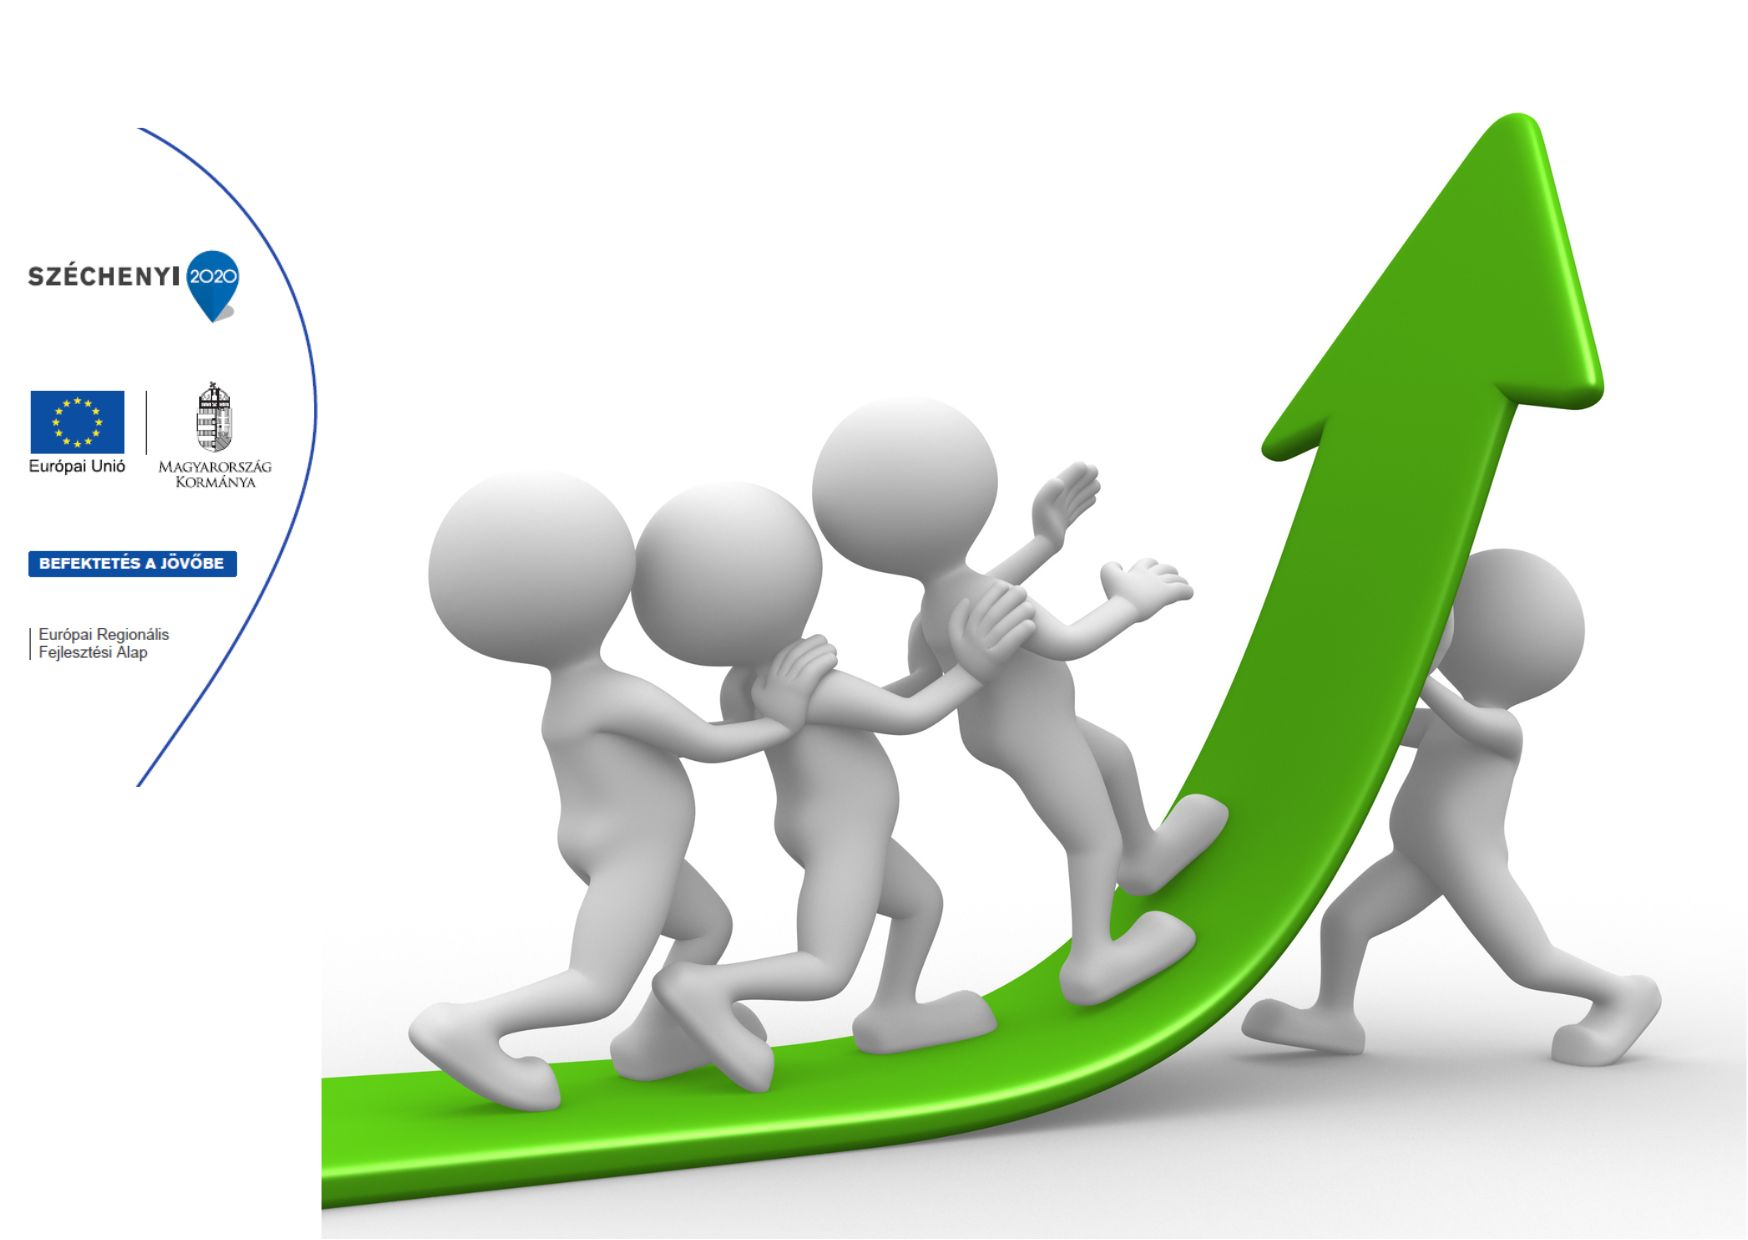
\includegraphics[width=70mm, keepaspectratio]{figures/inspiration.jpg}
    \caption{Inspiráció kreatív ábrázolása}
    \label {fig:inspiration}
\end{figure}
%----------------------------------------------------------------------------
